\documentclass[a4paper,10pt,epsf,fleqn]{article}
%\documentclass[a4paper]{jsarticle}
\setlength{\mathindent}{0mm}
%\usepackage[dvipdfm]{graphicx} 
%\usepackage{bmpsize}
\oddsidemargin=1cm\pagebreak[2]
\topmargin=-1cm
\setlength{\textwidth}{15cm}
\setlength{\textheight}{24cm}
\pagestyle{plain}
\usepackage{graphicx}	% required for `\includegraphics' (yatex added)
%\author{Takao Kotani}
%\title{ecalj --- Get statrted} 
\usepackage{setspace}
\usepackage{hyperref}
\usepackage{ulem}
\usepackage[usenames]{color}
\usepackage{makeidx}
\usepackage{ascmac}
%\bibliographystyle{apsrev4-1}
\setstretch{1.1}

%\newcommand{\fcode}[1]{\begin{screen} \verb@#1@ \end{screen}}
\newcommand{\rou}[1]{\noindent------------------------------------------------------------------------------------------------------------

\noindent{\bf \large #1}}
\newcommand{\fl}[1]{\noindent{\sf $\bullet$ #1\index{\sf #1}} : }
\newcommand{\fx}[1]{\subsection{\sf #1\index{\sf #1}}}
\newcommand{\ssx}[1]{\subsection{\bf #1\index{\bf #1}}}
\newcommand{\ssxx}[2]{\subsection{\bf #1\index{\bf #2}}}
\newcommand{\infiles}{\noindent\fbox{Input files}}
\newcommand{\outfiles}{\noindent\fbox{Output files}}
\newcommand{\GW}{$GW$}
\newcommand{\GWinput}{{\sf GWinput}\ }
\newcommand{\GWIN}{{\sf GWIN}\ }

\newcommand{\gbox}[1]{\noindent{\color{Green}\fbox{\parbox{260mm}{#1}}}}
\newcommand{\rbox}[1]{\noindent{\color{Red}\fbox{\parbox{260mm}{#1}}}}
\newcommand{\obox}[1]{\noindent{\color{Orange}\fbox{\parbox{260mm}{#1}}}}
\newcommand{\cyanbox}[1]{\noindent{\color{Cyan}\fbox{\parbox{260mm}{#1}}}}
\newcommand{\bluebox}[1]{\noindent{\color{Blue}\fbox{\parbox{260mm}{#1}}}}

\newcommand{\keyw}[1]{\fbox{\tt #1}}
\newcommand{\bfe}{{\bf e}}
\newcommand{\bfq}{{\bf q}}
\newcommand{\bfk}{{\bf k}}
\newcommand{\bfr}{{\bf r}}
\newcommand{\bfR}{{\bf R}}
\newcommand{\bfQ}{{\bf Q}}
\newcommand{\ds}{\displaystyle}

\newcommand{\exe}[1]{{\bf #1}}
\newcommand{\io}[1]{{\sf  #1}}
%\newcommand{\file}[1]{{\sf  #1}}
\newcommand{\raw}[1]{{\tt #1}}
\newcommand{\repp}[1]{p.\pageref{#1}}

\newcommand{\eiqr}{e^{i \bfq \bfr}}
\newcommand{\figp}[1]{\rotatebox{-90}{\includegraphics[width=10cm]{#1}}}

\newcommand{\bfex}{{\bf e}_x}
\newcommand{\bfey}{{\bf e}_y}
\newcommand{\bfez}{{\bf e}_z}
\newcommand{\bfa}{{\bf a}}
\newcommand{\bfb}{{\bf b}}
\newcommand{\bfT}{{\bf T}}

\newcommand{\bfS}{{\bf S}}
\newcommand{\bfiS}{{\it \Delta \bf S}}
\newcommand{\bfB}{{\bf B}}

\newcommand{\ispone}{\downarrow}
\newcommand{\isptwo}{\uparrow}

\newcommand{\eps}{\epsilon}
\newcommand{\D}{{\it \Delta}}
\newcommand{\scgw}{QS{\it GW} }

\newcommand{\req}[1]{Eq.(\ref{#1})}
\newcommand{\figss}[2]{\hspace{-3cm}\rotatebox{-90}{\includegraphics[width=6cm]{#1}}\rotatebox{-90}{\includegraphics[width=6cm]{#2}}}
\newcommand{\figs}[2]{\hspace{-2cm}\rotatebox{0}{\includegraphics[width=8cm]{#1}}\rotatebox{0}{\includegraphics[width=8cm]{#2}}}

\newcommand{\lmsuit}{{\tt lmsuit}\ }
\newcommand{\ecalj}{{\bf ecalj}\ }
\newcommand{\QSGW}{QSGW\ }
\newcommand{\ctrl}[1]{{\tt ctrl.{#1}}\ }

\newenvironment{mspace0}{\baselineskip=1mm}

\newenvironment{mspace}{\baselineskip=2mm}

\begin{document}
\baselineskip=6mm
\title{ ecalj method (detail for developments)\\ 
{\large \url{https://github.com/tkotani/ecalj}}}
%\date{April 2nd 2001}
\maketitle
\abstract{ xxxxxxxxxxx under construction xxxxxxxxxxxxxxx}
\noindent 
Methodological Details on the ecalj package. Refs.
\cite{kotani2015pmt} and \cite{kotani_quasiparticle_2014}.

\tableofcontents
\vspace{5mm}
\noindent$\bullet${\bf Reference}

\vspace{5mm}
\noindent$\bullet${\bf Index of I/O files, shel scripts and executions.}

\newpage
%\section{Software license agreement}
% ecalj is free for use, modify and redistribute.
% However, in any distribution of this codes, you have to
% clearly show thisection "Software licence agreement" in the pacakge.
% In any publications which uses (a part of) ecalj, 
% we need citation of the homepage of ecalj package
% https://github.com/tkotani/ecalj/ and lmsuite.


%%%%%%%%%%%%%%%%%%%%%%%%%%%%%%%%%%%%%%%%%%%%%%%%%%%%%%%%%%%%%%%%
\section{MEMO1xxx}

xxxxxxxxxxxxxxxxxxxxxxxxx MEMO xxxxxxxxxxxxxxxxxxxxxxxxxx\\

Co on MgO slab:
\begin{verbatim}
ecalj/MATERIALS/ctrl.mgoco
------from here ------------------
STRUC
     ALAT=1.88972687777
     PLAT=       3.00591       0.00000       0.00000000000  
                 0.00000       3.00591       0.00000000000 
                 0.00000       0.00000      16.00000000000 

SITE  ATOM=Mg       POS=   0.0000000   0.0000000   0.0000000  RELAX= 0 0 0
      ATOM=Mg       POS=   1.5029550   1.5029550   2.1723171  RELAX= 0 0 0
      ATOM=O        POS=   1.5029550   1.5029550   0.0000000  RELAX= 0 0 0
      ATOM=O        POS=   0.0000000   0.0000000   2.1032371  RELAX= 0 0 0
      ATOM=Co       POS=   0.0000000   0.0000000   4.1898024  RELAX= 0 0 1
      ATOM=Co       POS=   1.5029550   1.5029550   5.2139861  RELAX= 0 0 1
------to here ------------------


=== MAE by rotating crystal ===
--(we have a sample at
++(we have a sample at lm7K/TESTsmaples/MAEtest/, but only in GGA/LDA).


=== spin wave ===
  J calculation.
  

xxxxxxxxxxxxxxxx
   Recently, I renewed some part of algolism of GW/QSGW calculations
   (some ideas are taken from from PRB.81,125102(2010) 
    and Copmuter Physics Comm. 176(2007)1-13).
   ---> this is better than old versions; speed, memory (file size),
   and accuracy for anisortopic systems.
   For comparison, you can use old version in .git (gitk --all and check it out).
   See Copmuter Physics Comm. 176(2007)1-13).

xxxxxxxxxxxxxxxxxx
--------------------------------------------------------
-- QSGW: convergence check sheet.
--------------------------------------------------------
--1. Basis to expand eigenfuncitons. 
--   As for APW, try pwemax=3, 4, 5.
--   In principle, bigger is better.
--   Local orbitals for semicore were requied (for Fe, and so on).
--2. Re-expand eigenfuncions (QpGcut_psi for IPW part)
--   In principle, bigger is better. 
--3. Mixed product basis.  QpGcut_cou for IPW part. 
--   <ProductBasis> section for PB part.
--4. number of k points, Q0Pchoice(irrelevant but speed up).
--
--5. omg,dw  (bins to accumulate imaginary part).
--
--6. emax_sigm (use 2Ry to 6Ry. And see stability. In priniciple, bigger is better.) 
--
--7. Do GW with XCFUN=1 or 103 (VWN or GGA)?
--   In priniple, bigger emax_sigm reduce dependence on them.
--   But, not easy. We may take the difference as allowance of error.
  
  ------------------------------------
 
\end{verbatim}



%%%%%%%%%%%%%%%%%%%%%%%%%%%%%%%%%%%%%%%%%%%%%%%%%%%%%%%%%%%%55
\newpage
\section{Data structure and contents of files}

\baselineskip=4mm

\subsection{Basic i/o files to startr GW}
We need basic data set for the system and eigenfunctions
from which we start GW calculaitons. Note that \exe{lmchk} show crystal
structure informations.

1. Crystal structure.
   unit of lattice
   primitive cell 
   reciprocal cell
   atomic position
   point group symmetry
   
   core configuration.

2. q+G vectors.

3.  Eigenfunctions and eigenvalues.
  cutoffs of 



\fl{LATTC} Generated by \exe{echo 0$|$lmfgw}.
This contains the information of primitive translation vectors, lmxa and konf.
\label{lattc}
A sample is,
{\baselineskip=2.6mm
\begin{verbatim}
    10.26d0        ! alat       = lattice constant in a.u.
     0d0 .5d0 .5d0 ! plat(1:3,1)= 1st primitive translation vector in alat.
    .5d0 .0d0 .5d0 ! plat(1:3,2)= 2nd ...
    .5d0 .5d0 .0d0 ! plat(1:3,3)= 3rd ...
    -1d10 ! QpGcut_psi = maxmum of |q+G| in a.u. 
  -------------------------------------------
   2   4 ! nbas lmxax (max l for augmentation)
  -------------------------------------------
  -- ibas lmxa konf(s) konf(p) konf(d)... ----
      1   4   3   3   3   4   5
      2   4   3   3   3   4   5\end{verbatim}}
where negative {\tt QpGcut\_psi} in the 5th line means dummy.
True {\tt QpGcut\_psi} is given in GWIN0.
After "\verb#-- ibas lmxa konf(s) konf(p) konf(d)... ----#"
, you see numbers "\verb#3   3   3   4   5#" for
\verb#ibas=1#. These mean $3s, 3p ,3d, 4f, 5g$, which specify the lowest
principle quantum numbers of valence electrons. 
In other words, cores are $1s, 2s, 2p$ for \verb#ibas=1# in this case.
\vspace{5mm}

\fl{SYMOPS} \label{symops} Generated by \exe{echo 0$|$lmfgw}.
The point group operations. It is written through
{\baselineskip=2.6mm \begin{verbatim}
      open(file='SYMOPS')
      write(ifi,*) ngrp
      do ig = 1, ngrp
        write(ifi,*) ig
        do i=1,3
          write(ifi,"(3d24.16)") symops(i,1:3,ig)
        enddo
      enddo
      close(ifi)
\end{verbatim}}

\fl{CLASS} \label{class} Generated by \exe{echo 0$|$lmfgw}.
An example is;
{\baselineskip=2.6mm
\begin{verbatim}
      1  1
      2  1
      3  2
      4  2
\end{verbatim}}
The first numbers of each line are atomic-site number in the primitive cell.
(It should be the same as the line number). The second numbers of each line
are atomic classes for each atomic-site.\\

\fl{NLAindx} \label{nlaindx} Generated by \exe{echo 0$|$lmfgw}.\\
This file contains indexes 
($p_{\rm valence}, l, a$ ) for orbitals in the MT.
($p_{\rm valence}$ is radial function index, 
$a$ is atomic site index). Eigenfunctions are expanded in this order.
Usually we use LMXA=4, thus $l$ takes from 0 through 4.
An example is (two atoms in a cell); 
%This information is used to write {\sf GWIN\_V2.tmp}.
{\baselineskip=2.8mm
\begin{verbatim}
           NOTE: p=1,2,3 corresponds to phi,phidot,pz(local orbital)
     p  l   a    ilma  label(unused) 
----NLAindx start---------------
   105
     1  0   1     0    4S_p
     1  1   1     1    4p_p
     1  2   1     4    4d_p
     1  3   1     9    4f_p
     1  4   1    16    5g_p
     1  0   2    25    4S_p
     1  1   2    26    4p_p
     1  2   2    29    4d_p
     1  3   2    34    4f_p
     1  4   2    41    5g_p
     2  0   1    50    4S_d
     2  1   1    51    4p_d
     2  2   1    54    4d_d
     2  3   1    59    4f_d
     2  4   1    66    5g_d
     2  0   2    75    4S_d
     2  1   2    76    4p_d
     2  2   2    79    4d_d
     2  3   2    84    4f_d
     2  4   2    91    5g_d
     3  2   1   100    3d_l
\end{verbatim}
}
(last labels,4S\_p... are just for memo. p,d,l means radial function
index 1,2, 3(first column $n$).)\\

\fl{ldima} Generated by \exe{echo 0$|$lmfgw}.
Number of LMXA**2 for atomic sites.
(this is used only from \exe{hqpe\_sc}---QSGW mode; this infomation is
also in other files such as \io{LATTC}; we currently only allow all LMXA
should be the same).\\

\fl{ves*} Generated by \exe{echo 0|lmfgw}.
Electro static potential \exe{lmf} or \exe{echo 1$|$lmfgw}.
(only for the bandoffset calculaitons.)\\

\fl{rhoMT*}
Radial electron density within MT \exe{echo 1$|$lmfgw}.\\
(used only for spin susceptibility mode in fpgw/main/hbasfp0.m.F---fpgw/gwsrc/basnfp.F).\\

\fl{QGpsi,QGcou} generated by \exe{echo 1$|$qg4gw}.\\
IPW for psi and for coulomb interaction.
See the last part of \io{lqg4gw}.
This is written by fpgw/main/qg4gw.F-gwsrc/mkqg.F.
Search file handles of them, ifiqg and ifigqc in mkqg.F

\begin{verbatim}
mkqg.F; Let us search ifiqg.
  This routine generates all required q points and G for q by QpGcut_psi,QpGcut_cou.
-------
      write(ifiqg ) nqnum,ngpmx,QpGcut_psi,nqbz,nqi,imx,nqibz
      write(ifiqgc) nqnum,ngcmx,QpGcut_cou,nqbz,nqi,imxc

      allocate( ngvecprev(-imx:imx,-imx:imx,-imx:imx) )       !mar2012takao
      allocate( ngveccrev(-imxc:imxc,-imxc:imxc,-imxc:imxc) ) !mar2012takao
      ...
      do iq = 1, nqnum
         q = qq(1:3,iq)
         ...
         write (ifiqg) q, ngp, irr(iq)
         write (ifiqg)  ngvecp,ngvecprev !ngvecprev is added on mar2012takao
         write (ifiqgc) q, ngc
         write (ifiqgc) ngvecc,ngveccrev
      enddo
      write(6,*) ' --- Max number of G for psi =',ngpmx
      write(6,*) ' --- Max number of G for Cou =',ngcmx
-------------------------------
NOTE:
      ngvecp(1:3,1:ngp)   : G vector for phi, integer qlat unit
      ngvecc(1:3,1:ngp)   : G vector for cou, integer qlat unit
      ngvecprev(n1,n2,n3) : inversion table
      ngvecprec(n1,n2,n3) : inversion table
      nqnum:   total number of q points.
      nqbz:    number of q point in the BZ
      nqibz:   number of irrducible q points of regular mesh (read from QIBZ).
      nqi:     number of irreducible points including offset Gamma points. 
               We calcualte eigenfunction and Vxc only for these points.
      irr(iq): irreducible point or not. For irr=1, calculate eigenfuncions.
      imx:     to allocate ngvecprev as follows.
    ----------------------
      alat :   unit of length (in a.u.).
      plat(3,3): primitive lattice vectors in the unit of alat
      qlat(3,3): invese lattice vector of plat. \delta_ij = sum(plat(:,i)*qlat(:,j))
    -------------------------------
      q+g(1:3,iq,ig) = 2*pi/alat*( q(1:3,iq)+sum(qlat(1:3,:)*(ngvecp(:,ig))) )
                      ,where iq=1,nqnum and ig=1,ngp(iq).
    -----
    Inverse mapping is
      ngvecp(1:3,ig)= ngvecprev(ngvecp(1,ig),ngvecp(2,ig),ngvecp(3,ig))
\end{verbatim}
\ \\


%%%%%%%%%%%%%%%%
\fl{DATA4GW\_V2} Crystal structures and so.\\
Generatege by lmf2gw, and read by rdata4gw\_v2.

\begin{verbatim}
----------------------------
     & nsp,      ! =1 or 2, corresponding to para or ferro.
     & nbas,     ! Number of atom in the primitive cell
     & nclass,   ! Dummy. =natom=nbas in the current code.
                         
     & nrmx,     ! = maxval(nr(1:nclass))  Maximum number of nr
     & ncoremx,  ! = maxval(ncore(1:nclass))
c
     & lmxamx,   ! = maxval(lmxa(1:nclass))
     & ngpmx,    ! Maximum number of G vector.
     & nband,    ! Number of bands given by GWIN0
     & ldim,     ! = sum ( (lmxa(1:nbas)+1)**2 )
     & ldim2,    ! = total number of augmentation functions nRlm (total of NLAindx).
     & nphi,     ! = total number of augmentation functions nRl  
     & nqbze     ! = nqbz*(1+nq0i). Number of q points given by qg4gw

nindx(ldim2),lindx(ldim2),ibasindx(ldim2): nla index shown in NLAindx

---------------
Cell DATA:
alat: unit
plat: primitive vector
qbze(3,nqbze): q vector.
efermi: fermi energy

---------------
ATOMIC DATA:
iclass(ibas)=ibas: dummy
aa(nclass),bb(nclass): specify radial mesh. r(i)=b(exp((i-1)*a)-1)
bas(3,nbas): atomic position
lmxa_d(nclass): LMXA (in the current version. all LMXA should be the same.
nr(nclass): radial mesh
konf(0:lmxa): principle quantum number of valence electron.
ncore_d(nclass): number of cores.

 CORE:
ec_d(ncoremx, nclass, nsp),  : core eigenvalue
gx_d (nrmx, 0:lmxamx, nphimx,  nclass,nsp): valence radial function
gcore_d(nrmx, ncoremx, nclass,nsp) core radial funciton.

 VAL:
evl_d (nbandmx, nqbze, nsp) : valence eigenvalue
vxclda(nbandmx, nqbze, nsp): LDA Vxc

---------------
Coefficients:
cphi(ldim2,nbandmx,nsp,nqbze): Coefficient of eigenfunciton within MTs. See NLAindx.
geig(1:ngp,1:nbandmx,nsp,nqbze): Coefficient of eigenfunciton for IPW exp(i q+G r).



This is a head part of lmf2gw
Cr--- From DATA4GW_V2 -----
Cr   nbas            : the number atom in the primitive cell
c
Cr  alat        : lattice constant in a.u.
Cr  plat(1:3,1) : 1st primitive translation vector in the unit of alat
Cr  plat(1:3,2) : 2nd primitive translation vector
Cr  plat(1:3,3) : 3rd primitive translation vector
c
c-- eigenfunctions for all q points.
Cr  evl (1:nband)          :  eigenvalue
Cr  cphi(1:ldim2,1:nband) : the coefficienets of eigenfunction for phi(augmentation wave)
Cr  geig(1:ngp,  1:nband) : the coefficienets of eigenfunction for IPW
Cr
Cr   nindx   (1;ldim2) : n index (phi=1 phidot=2 localorbital=3)
Cr   lindx   (1:ldim2) : l index
Cr   ibasindx(1:ldim2) : ibas index . These are used to re-ordering cphi.
Cr                     :  mindx(1:ldim2)  is generated under the asuumption that
Cr                        m=-l:l is successively ordered.
Cr
Cr  vxclda (1:nband) : lda XC potential <psi|Vxc(n)|psi> for each eigenfunctions
c
c--   Atomic data for all the atom in the cell, ibas=1,nbas
Cr   Z:
Cr   nr a,b; mesh is r(i)=b*(exp(a(i-1))-1)
Cr   ncore: number of core.
Cr   ec(1:ncore)
Cr   gx : radial wave function phi.
\end{verbatim}

lmf2gw:
\io{CphiGeig}
          write(ificg) cphi(1:ldim2,1:nbandmx)

          write(ificg) ngp
          write(ificg) geig(1:ngp,1:nbandmx)

\io{VXCFP.chk} Eigenvalue and Vxc check. only for check\\

\newpage
\section{spin susceptibility (old memo)}

%%%%%%%%%%%%%%%%%%%%%%%%%%%%%%%%%%%%%%%%%%%%%%%%%%%%%%%%%%%%%%%%%%%%%%%%%%%%%%%%%%%%%%
\newpage

\subsection{transverse spin susceptibility $\chi^{+-}$ calculation} 
\label{chipmcal}
[I changed sign of $\chi$! (July2007); This definition may be different from other text book. Be careful]
The non-interacting transverse spin susceptibility 
$\chi^{0+-}(\bfr,\bfr',t-t')$ is given as
\begin{eqnarray}
\chi^{0+-}(\bfr,\bfr',t-t') = 
-i\langle T(S_+(\bfr,t) S_-(\bfr',t') \rangle
=- i G_\isptwo(\bfr,\bfr',t-t') G_\ispone(\bfr',\bfr,t'-t) 
\label{generalchi0t}
\end{eqnarray}
for non-interacting system (Lindhard-like poralization function).
In $\omega$ space, this reduced to
\begin{eqnarray}
&&\chi^{0+-}(\bfr,\bfr',\omega) \nonumber \\
%= 
%  G_\isptwo(\bfr,\bfr',\omega) \otimes G_\ispone(\bfr,\bfr',-\omega) 
%=
%    G^{\rm e}_\isptwo(\omega) \otimes G^{\rm h}_\ispone(-\omega) 
%  + G^{\rm h}_\isptwo(\omega) \otimes G^{\rm e}_\ispone(-\omega)   \nonumber \\
&&= 
\sum^{\rm  occ}_{n \ispone} \sum^{\rm  unocc}_{n'\isptwo}
\frac{
\Psi_{n\ispone}^*(\bfr)      \Psi_{n'\isptwo}(\bfr)
\Psi_{n'\isptwo}^*(\bfr') \Psi_{n\ispone}(\bfr') 
}{\omega-(\epsilon_{n'\isptwo}-\epsilon_{n\ispone})+i \delta} 
+ \sum^{\rm  unocc}_{n \ispone} \sum^{\rm occ}_{n'\isptwo}
\frac{
\Psi_{n\ispone}^*(\bfr)      \Psi_{n'\isptwo}(\bfr)
\Psi_{n'\isptwo}^*(\bfr') \Psi_{n\ispone}(\bfr') 
}{-\omega-(\epsilon_{n\ispone}-\epsilon_{n'\isptwo})+i \delta},
\label{generalchi0}
\end{eqnarray}
%where $\otimes$ means convolution as for $\omega$;  $f(\omega) \otimes g(\omega)
%= \int_{-\infty}^{\infty} \frac{i d \omega}{2\pi} f(\omega-\omega') g(\omega')$.
Here $\ispone$ is for majority ({\tt isp=1}) and 
$\isptwo$ is for minority ({\tt isp=2}), 
$\left(
 \begin{array}{c} {\rm isp=1} \\ 
                  {\rm isp=2} 
  \end{array}   
\right) =
\left(
 \begin{array}{c} \ispone \\ 
                 \isptwo 
  \end{array}   
\right)$. \\
   
\noindent $S^+(\bfr) = \Psi_{\rm isp=1}^*(\bfr) \Psi_{\rm isp=2}(\bfr) 
= \Psi_{\rm \ispone}^*(\bfr) \Psi_{\rm \isptwo}(\bfr)$, 

\noindent $S^-(\bfr') = \Psi_{\rm isp=2}^*(\bfr') \Psi_{\rm isp=1}(\bfr') 
= \Psi_{\rm \isptwo}^*(\bfr') \Psi_{\rm \ispone}(\bfr')$, \ 



\noindent Notes:
\begin{itemize}
\item This definition of $\chi^{0+-}$ 
results in $\chi^{0+-} \to \frac{\rm m}{\omega-\Delta_{\rm ex}}$
at ${\bf q}=0$ in the case of shifted-band model as 
$\epsilon_\bfk^\isptwo = \epsilon_\bfk^\ispone + \Delta_{\rm ex}$.
Here $\Delta_{\rm ex}$ means exchange splitting, and $m = N_\ispone- N_\isptwo$.
For paramagnetic case, this definition gives $\chi_0 = 2 \chi^{0+-}$, where
 $\chi_0$ is usual Lindhard polarization function for density response.
%(Because of this, our program rather show $-\chi^{0+-}$ in {\tt \bf ChiPM*} file.

\item Recall 
$ e^{-i (\eps-\eps') t} \theta(t)  = e^{-i \eps t} \theta(t) \times e^{+i \eps' t} \theta(t)$ 
or equivalently 
$ \frac{1}{\omega-(\eps-\eps')+i \delta}= \int d\omega' \frac{1}{\omega-\omega'-\eps+i \delta} \frac{1}{-\omega'-\eps'-i \delta}$.

\item If no occupation for minority channel, only the 1st term in \req{generalchi0} remains.
In contract to charge density, $\chi^{0+-}$ is not symmetric for $\omega \leftrightarrow -\omega$. 
\end{itemize}

By the way, the physically meaningful quantity is the retarted verion of $\chi^{0+-}$,
named as $\chi^{0+-}_{\rm Ret}$, which is given by changing the sign of $+ i \delta$ in \req{generalchi0}
so as to make it propotional to $\theta(t)$.
Let us assume colinear case (z-axis), 
and consider adding external transversal magnetic fiels $B_x(\bfr,t)$ and $B_y(\bfr,t)$ 
for our system. For non-interacting system, this $\chi^{0+-}_{\rm Ret}$ 
specify the linear repsonse to such $B_x$ and $B_y$.
Instead of them, it is convenient to use the complex field, $b^- = b_x -i b_y$,
(I introduce ${\bf b}$ in unit of 
$g \mu_{\rm B}/2$, so that $(g \mu_{\rm B}/2) B_x =  b_x$:
electron's spin magnetic momenets is $-2 g \mu_{\rm B} {\bf s}$.)
Then the additional Hamiltonian due to this magnetic field is written
as 
\begin{eqnarray}
H_{\rm ext\_mag} 
&=&  \int d^3r B(\bfr) \cdot g \mu_{\rm B} {\bf s}(\bfr)
=  2 \int d^3r {\bf b}(\bfr) \cdot {\bf s} (\bfr) \nonumber \\
&=&  \int d^3r \left[ b^+(\bfr) s^-(\bfr) + b^-(\bfr)s^+(\bfr) 
+ 2 b_z(\bfr) s_z(\bfr) \right],
\end{eqnarray}
where $s^-(\bfr) = s_x(\bfr)- i s_y(\bfr)$ and so on.
$\ds s_x(\bfr) = \sum_{\alpha,\beta} 
\langle \hat{\psi}^\dagger_\alpha(\bfr) \frac{1}{2} \sigma^x_{\alpha \beta}
\hat{\psi}_{\beta}(\bfr) \rangle $
and so on, where $\sigma^x_{\alpha \beta}$ is the Pauli matrix.
The induced spin moment $\D s^-$ for non-interacting system is given as
\begin{eqnarray}
&& \D s^-(\bfr,t) = \int dt' d^3r' \! \chi^{0+-}_{\rm Ret}(\bfr,\bfr',t-t') b^-(\bfr',t').
\end{eqnarray}
[because of $\theta(t)$ in  $\chi^{0+-}_{\rm Ret}$, $t-t'>0$.].

In the case of interacting system, we need to construct $\chi^{+-}$.
We define ${U}(\bfr,\bfr',\omega)$ as
\begin{eqnarray}
(\chi^{+-})^{-1} =  \left(\chi^{0+-}\right)^{-1} - {U}.
\label{chirpa0}
\end{eqnarray}
This is taken as the definition of ${U}(\bfr,\bfr',\omega)$.
How to define $U$ is the problem --- See my {\bf spin wave paper} in Arxiv.
We utilize one degree of freedome per atom (so $\chi^{+-}$ is 
the matrix whose dimension is the number of magnetic atoms), and sum rule.
(Some one may call this approximation as ``rigid moment approximation''.
 But it can be misleagind. Be careful about what I did.


\noindent ----MEMO----------------------\\
{\bf \tt eps\_lmfh\_chipm}: Our fpgw code can calculate
$\chi^{0+-}$ in this form of expansion
\begin{eqnarray}
\chi^{0+-}(\bfr,\bfr',\omega) 
= \frac{1}{N}\sum_q \chi^{+-}_\bfq(\bfr,\bfr',\omega)
= \frac{1}{N}\sum_q \sum_I \sum_J
M^\bfq_I(\bfr) \chi^{0+-}_{\bfq IJ}(\omega) (M^\bfq_J(\bfr'))^*.
\label{chiexpand}
\end{eqnarray}
Here $\{ M^\bfq_I(\bfr) \}$ is the complete set with the periodicity specified 
by $\bfq$ (Mixed basis).
In other words, $\{ M^\bfq_I(\bfr) /e^{i \bfq \bfr} \}$ 
is the complete set to expand periodic function.
However, I have not used this now...;problem is determination of $U$. How to do it?
(sum rule is not enough. we need static response?).


\subsubsection{Sum rule(moment)} 
The equation of motion of spin is written as
\begin{eqnarray}
i \dot{\hat{\bf S}} = [\hat{\bf S},  \hat{H}]
\end{eqnarray}
\begin{eqnarray}
\chi^{+-}(\bfr,\bfr',t-t') 
&=& -i\langle T\left( S_+(\bfr,t) S_-(\bfr',t') \right) \rangle                \nonumber\\
&=& -i\langle S_+(\bfr,t)   S_-(\bfr',t') \rangle \theta(t-t')
+ i\langle S_-(\bfr',t') S_+(\bfr,t)   \rangle \theta(t'-t)
\end{eqnarray}
Thus
\begin{eqnarray}
&&\frac{\partial }{\partial t} \chi^{+-}(\bfr,\bfr',t-t') 
= -i [S_+(\bfr,t),   S_-(\bfr',t)] \delta(t-t') \nonumber\\
&&-  \langle [S_+(\bfr,t),H]   S_-(\bfr',t') \rangle \theta(t-t') 
+  \langle S_-(\bfr',t')   [S_+(\bfr,t),H] \rangle \theta(t'-t),
\end{eqnarray}
where $[S_+(\bfr,t), S_-(\bfr',t)]= 2S_z(\bfr,t) \delta(\bfr-\bfr')$.
As $\int d^3r [S_+(\bfr,t),H]=0$, we have
\begin{eqnarray}
&&\int d^3r \frac{\partial }{\partial t} \chi^{+-}(\bfr,\bfr',t-t') 
= -i \langle [S_+(\bfr,t),   S_-(\bfr',t)] \rangle \delta(t-t') 
= -2 i \langle S_z(\bfr,t) \rangle \delta(t-t') 
\end{eqnarray}
This reads
\begin{eqnarray}
&&\int d^3r \omega \chi^{+-}(\bfr,\bfr',\omega) 
= 2 \langle S_z(\bfr',t) \rangle = M_z(\bfr') 
\end{eqnarray}

\noindent $\bullet$ At $\omega \to \infty$, this condition get stronger as
\begin{eqnarray}
\chi^{+-}(\bfr',\bfr,\omega) \to
\frac{M(\bfr)}{\omega} \delta(\bfr-\bfr') + O(1/\omega^2).
\label{summ2}
\end{eqnarray}
See {\bf spin wave paper}.


\subsubsection{Rigid moment approximation} 
This means that ``the magnetic moments are very rigid that they
changes without changing its form''. 
In other words, $\D s^-(\bfr)$ induced by any $b_-(\bfr)$ 
are propotional to its original moment $s_z(\bfr)$.
Rigid rotation in spin space can be expressed by e.g.,
$\ds U^x(\theta)=\exp\left( \frac{i \sigma^x \theta}{2}\right)$ in the case of x-axis rotation.
Then you can easily verify
$(U^x(\theta))^\dagger \sigma^z U^x(\theta) \propto \sigma^y$
This means $\D s^-(\bfr) \propto s_z(\bfr)$. 
Note that we did rotation only in spin space.
We neglect the mappling of $\bfr$ when we rotate spin---this will cause
little problem when the moment is rather spherical.
Be careful; our approximation (one-degree of freedom per magnetic atom) 
may be a little different from the ``rigid moment approximation''.
I did not want to mix it up, thus I avoided this terminology in my {\bf [spin wave paper]}.



%% %%%%%%%%%%%%%%%%%%%%%%%%%%%%%%%%%%%%%
%% \newpage
%% \begin{figure}[ht]
%% %\begin{center}
%% \vspace{-3cm}

%% \figs{SpinNi_000013_line100.eps}{SpinNi_000017_line100.eps}

%% \figs{SpinNi_000020_line100.eps}{SpinNi_000022_line100.eps}

%% %\end{center}
%% \caption[]{ Ni-100(a=6.640(experimental) or 6.481(da159---LDA value) a.u.)$\times$(LDA or \scgw) :  
%% {$\ds {\rm Im} \left[ \frac{\langle m| \chi^{+-} |m \rangle}{\langle m|m \rangle^2} \right]$.}
%% We used Eq.(\ref{chieq}),Eq.(\ref{chiinv}) and Eq.(\ref{chipmnolfc}) (Without LFC).}
%% \label{Nichipmnolfc100}
%% \end{figure}

%% \newpage
%% \begin{figure}[ht]
%% %\begin{center}
%% \vspace{-3cm}

%% \figs{SpinNi_000015_line111.eps}{SpinNi_000018_line111.eps}

%% \figs{SpinNi_000021_line111.eps}{SpinNi_000023_line111.eps}

%% %\end{center}
%% \caption[]{ Ni-111. Same as Fig.\ref{Nichipmnolfc100}.}
%% \label{Nichipmnolfc111}
%% \end{figure}


%% %%%%%%%%%%%%%%%%%%%%%%%%%%%%%%%%%%%%%%%%%%%%%%%%%%%%%%%%%%%%%%%%%%%%%%%
%% \newpage
%% \begin{figure}[ht]
%% %\begin{center}
%% \vspace{-3cm}

%% \figs{SpinFe_000025_line100.eps}{SpinFe_000027_line100.eps}

%% \figs{SpinFesc_line100.eps}{SpinFesc_da197_line100.eps}

%% %\end{center}
%% \caption[]{ Fe-100(a=5.408(experimental) or 5.211(da197---LDA value) a.u.)$\times$(LDA or \scgw) :  
%% {$\ds {\rm Im} \left[ \frac{\langle m| \chi^{+-} |m \rangle}{\langle m|m \rangle^2} \right]$.}
%% We used Eq.(\ref{chieq}),Eq.(\ref{chiinv}) and Eq.(\ref{chipmnolfc}) (Without LFC).}
%% \label{Fechipmnolfc100}
%% \end{figure}


%% %%%%%%%%%%%%%%%%%%%%%%%%%%%%%%%%%%%%%%%%%%%%%%%%%%%%%%%%%%%%%%%%%%%%%%%
%% \newpage
%% \begin{figure}[ht]
%% %\begin{center}
%% \vspace{-3cm}

%% \figs{SpinFe_000026_line110.eps}{SpinFe_000028_line110.eps}

%% \figs{SpinFesc_line110.eps}{SpinFesc_da197_line110.eps}
%% %SpinFe_000032_line110.eps}

%% %\end{center}
%% \caption[]{ Fe-110. Same as Fig.\ref{Fechipmnolfc100}.}
%% \label{Fechipmnolfc110}
%% \end{figure}



%%%%%%%%%%%%%%%%%%%%%%%%%%%%%%%%%%%%%%%%%%%%%%%%%%%%%%%%%%%%%%%%%5
%\newpage
\subsubsection{static $J(q)$ calculation---- Heisenberg Model}
(See kotani's SW paper).
The total energy of our spin system is assumed to be
\begin{eqnarray}
&& {\cal H} = - \sum_{Rn} \sum_{R'n'} 
J_{Rn R'n'} \bfS_{Rn} \cdot \bfS_{R'n'} + g \mu_B \sum_{Rn} 
\bfS_{Rn} \cdot \bfB_{Rn}
\label{hei1}
\end{eqnarray}
. Here we take all site indexes $Rn$ and $R'n'$ 
($J_{RnRn}=0$. $J_{RnR'n'}=J_{R'n'Rn}$. 
It we restrict sum as $Rn>R'n'$, factor 2 appears.).
$\bfS_{Rn}$ is the spin at $Rn$ ($R$ is for primitive cell, $n$ specify
site in a cell).
The equation of motion 
$-i\hbar \dot{\bfS}_{Rn} = [{\cal H} , {\bfS}_{Rn}]$,
is reduced to be
\begin{eqnarray}
\hbar \dot{\bfS}_{Rn} = \bfS_{Rn} \times 
\left(2 \sum_{R'n'} J_{Rn R'n'} \bfS_{R'n'} - g \mu_B \bfB_{Rn} \right)
\label{hei2}
\end{eqnarray}
We introduce $g \mu_B \bfB = 2 \bfb$, and $\bfS_{Rn}=\bfS_{Rn}^0 + 
\bfiS_{Rn}$. Then \req{hei2} reduce to
\begin{eqnarray}
&&\hbar \dot{\bfiS}_{Rn} =  \bfS^0_{Rn} \times
\left(2 \sum_{R'n'} J_{Rn R'n'} \bfiS_{R'n'}  \right)
+ \bfiS_{Rn} \times 
\left(2 \sum_{R'n'} J_{Rn R'n'} \bfS_{R'n'} \right)
- 2 \bfS^0_{Rn} \times \bfb_{Rn} \nonumber \\
&&= \sum_{R'n'} \left(2 \bfS^0_{Rn} J_{Rn R'n'} \right) \times \bfiS_{R'n'}
- 
\left(2 \sum_{R'n'} J_{Rn R'n'} \bfS^0_{R'n'} \right)  \times \bfiS_{Rn} 
- 2 \bfS^0_{Rn} \times \bfb_{Rn} 
\label{hei3}
\end{eqnarray}
Introduce the fourier transformation as
$\bfiS_{Rn} = \frac{1}{N} \sum_\bfk \bfiS_n(\bfk) e^{i \bfk \bfR}$.
Then \req{heis3} reduce to
\begin{eqnarray}
&&\hbar \dot{\bfiS}_{n}(\bfk)   
= \sum_{n'} \left( 2 \bfS^0_{n} J_{n n'}(\bfk) 
- \left(2 \sum_{n''} J_{n n''}(0) \bfS_{n''}^0\right) \delta_{nn'}\right)  \times \bfiS_{n'}(\bfk)
- 2 \bfS^0_{n} \times \bfb_{n}(\bfk).
\label{hei4}
\end{eqnarray}
Assume $\ds {\bfiS}_{n}(\bfk) \propto e^{-i \frac{\omega t}{\hbar}}$,
we have 
\begin{eqnarray}
 \sum_{n'} \left(\frac{i \omega \delta_{nn'}}{2} +  \bfS^0_{n} J_{n n'}(\bfk) 
- \left( \sum_{n''} J_{n n''}(0) \bfS_{n''}^0\right) \delta_{nn'}\right)  \times \bfiS_{n'}(\bfk)
= \bfS^0_{n} \times \bfb_{n}(\bfk).
\label{hei5}
\end{eqnarray}
Let us consider colinear ground state, then $\bfS^0_{n}= S_n \bfe_z$
($S_n$ is the size of spin with sign). You have
\begin{eqnarray}
\sum_{n'} \left( \frac{i \omega \delta_{nn'}}{2S_n} \right) \bfiS_{n'}(\bfk)
+\sum_{n'} \left( J_{n n'}(\bfk) 
- \left( \sum_{n''} \frac{1}{S_n} J_{n n''}(0) S_{n''} \right) \delta_{nn'}\right)  \bfez \times \bfiS_{n'}(\bfk)
=  \bfez \times \bfb_{n}(\bfk).
\label{hei6}
\end{eqnarray}
As $\bfS = S^+ \frac{\bfex -i \bfey}{2}
         + S^- \frac{\bfex +i \bfey}{2} + S^z \bfez$,
and $\bfez \times ({\bfex \pm i \bfey}) = \mp i({\bfex \pm i \bfey})$
we have,
\begin{eqnarray}
&&\sum_{n'} \left( \frac{\omega \delta_{nn'}} {2S_n} -
 \bar{J}_{n n'}(\bfk) \right)  S^+_{n'}(\bfk)
=  b^+_{n}(\bfk). \\
&&\sum_{n'} \left( \frac{\omega \delta_{nn'}} {2S_n} + 
\bar{J}_{nn'}(\bfk)  \right)    S^-_{n'}(\bfk)
=  b^-_{n}(\bfk),
\end{eqnarray}
where
\begin{eqnarray}
\bar{J}_{nn'}(\bfk)=  J_{n n'}(\bfk) 
- \left( \sum_{n''} \frac{1}{S_n} J_{n n''}(0) S_{n''} \right) \delta_{nn'}
\label{jbar}
\end{eqnarray}
This $\bar{J}_{nn'}(\bfk)$ and also $S_n $ are stored in \verb#Jmat# file
(or \verb#JMAT# line when you run a script \verb#ecal/util/calj\_summary_mat# 
which calls (\verb#calj_nlfc_mat#). 
Only the differenc between $\bar{J}_{nn'}(\bfk)$ and $J_{n n'}(\bfk)$
are diagonal parts. 
These are determined so that $\int d^3k {J}_{nn}(\bfk)=0$.\\

\noindent JJMAT contains another definition of $J$, which is to reproduce SW spectrum
(but it does not work well in cases because the SW peaks are not well identified at high $\bfk$.)\\

See my spin wave paper.


\subsubsection{$J(q)$ and Tc}
---- this section is my memo. Not need to read here ----

(This section is not consistent with previous page. Only a case, with an atom in the cell).
The total energy of our spin system is assumed to be
\begin{eqnarray}
&& E_{\rm spin} = - \sum_i \sum_j J_{ij} \bfe_i \cdot \bfe_j
\label{heis1}
\end{eqnarray}
. Here we take all site indexes $i$ and $j$ 
($J_{ii}=0$. $J_{ij}=J_{ji}$. 
It we restrict sum as $i>j$, factor 2 appears.).
$\bfe_i$ is the unit vector to specify the spin direction.

%% $\chi^{+-}(\bfq) \equiv \chi^{+-}(\bfq, \omega=0)$
%% gives the static energy difference for the spin system 
%% within the linear response scheme. 
%% Consider the linear response based on \req{heis1}, 
%% $J(\bfq)$ should satisfy
%% \begin{eqnarray}
%% J(\bfq) - J(0) = -\langle m| \left( \chi^{+-}(\bfq) \right)^{-1} |m \rangle 
%% =
%% - \langle m| \left( \chi^{0+-}(\bfq) \right)^{-1} |m \rangle 
%% + \langle m| I |m \rangle.
%% \label{jdiff}
%% \end{eqnarray}
%% Here we used Eq.(\ref{chieq}) and 
%% $\langle m| I |m \rangle= \langle m|
%% \left( \chi^{0+-}(\bfq=0,\omega=0) \right)^{-1}|m \rangle$
%% as in Eq.(\ref{sp0cond}).

If we identify $ E_{\rm spin}$ as the Heisenberg hamiltonian
with a fixed spin moment $m = N^{\ispone}- N^{\isptwo}$,
the spin wave dispersion is given as
\begin{eqnarray}
\omega_\bfq = \frac{4}{m} \left[ J(0) -J(\bfq) \right].
\label{omegaq}
\end{eqnarray}
This $\omega_\bfq$ is different from the true pole of 
$\langle m| \left( \chi^{+-}(\bfq,\omega) \right)^{-1} |m \rangle$ 
 except
$\bfq \to 0$.

The critical temperature $T_{\rm c}$ is given as
$T_{\rm c} = \frac{2}{3} J(\bfQ) Q_{\rm factor}$.
This $Q_{\rm factor}$ can be $(S+1)/S$, but 
it seems to be taken as unity usually...
$J(Q=0)$ is for ferromagnetic case.

In order to calculate $J(0)$,
integrate the left hand side of Eq.(\ref{jdiff}) in the BZ
and use $\ds \int \frac{\Omega d^3 q}{2 \pi} J(\bfq)=0$. It gives

\begin{eqnarray}
T_{\rm c} = \frac{2}{3} J(0) = 
\frac{2}{3} \int \frac{\Omega d^3 q}{2 \pi}
\langle m| \left( \chi^{+-}(\bfq) \right)^{-1} |m \rangle 
= 
\frac{2}{3} \frac{m}{4} \int \frac{\Omega d^3 q}{2 \pi} \omega_\bfq 
\label{tceq}
\end{eqnarray}

This equation contains two probrems.
\begin{enumerate}
\item[(1)] Mapping to a Heisenberg model.\\
This may cause a problem in the case of transition metals, and so.
The spin waves have strong dumping.
Further, we don't include the temperature-dependence of the model itself.

%$\omega_\bfq$ around BZ boundaries can be
%very different from \req{omegaq}.
%However, this mapping may be not so problematic for insulators---
%no Stonar dumping case (exactly speaking, no dumping channel to quasi particle pairs).\\
%For Ni, ${omegaq} \approx$ 800 meV at q=(100), 
%though the spin-wave spectrum has rather sharp peak around 550meV 
%(the peak is originally from the structure of $Im(\chi_0(\omega))$).
%For Fe, it shows 


\item[(2)] Mean field apprximation to solve the Heisenberg model.\\ 
In other words, $Q_{\rm factor}$ should be a functional of $J(\bfq)$ for all $\bfq$.
We can devide the problem into classical part and quantum part.
A contraversial point is that the integral in \req{tceq} 
is rather dominanted by the contribution around the BZ boundaries,
though we can expect that $T_{\rm c}$ can be rather strongly controlled
by low energy $\omega_\bfq$. 

\end{enumerate}

~\\

--- (this is what Mark says)---

[MF Quantum Tc] --- too high.  (S+1)/S * MFC

[Full Quantum Tc] --- Exact solution of the Heisenberg Model.
 
[MF Classical Tc] 

[Full Classical Tc] (probably $\sim$ 80 \% of MFC)



%%%%%%%%%%%%%%%%%%%%%%%%%%%%%%%%%%%%%%%%%%%%%%%%%%%%%%%%%%%%%%%%%%%%%%%
\begin{figure}[hbpt]
\begin{center}
\includegraphics[width=10cm]{ZBmnasw1.eps}
\end{center}
\caption[]{
$\omega_\bfq$ for ZincBlend MnAs by Eq.\ref{omegaq}. 
LDA case vs. \scgw case. 
\scgw makes ZincBlend MnAs as half-metallic. 
m denotes on-site moment in $\mu_B$. 
The mean-filed $T_c$ in \scgw is about 600 K.
{\large NOTE: not yet published. We have to re-examine this!!!}}
\label{zbmnas}
\end{figure}


\newpage
\section{Memo({Method and Equations})}

\vspace{1cm}
\noindent {\bf Hilbert transformation}(called as Sergey mode) ):\\
This is standard calculation now.
Our standard version (a script {\bf gw\_lmfh, gwsc}) is with
the Hilbert transformation (Kramers-Kr\"onig relation).
We first calculate only the imaginary part of $\Pi$
Then we get full $\Pi$ through the Hilbert transformation.
In other words, we calculate the imaginary part of $\Pi$ by replacement of\\
$\left(\frac{1}{\omega-\epsilon_{{\bf q+k}n'}+\epsilon_{{\bf k}n}+i \delta}
-\frac{1}{\omega+\epsilon_{{\bf q+k}n'}-\epsilon_{{\bf k}n}-i \delta}\right)$
with $\delta(\omega-\epsilon_{{\bf q+k}n'}+\epsilon_{{\bf k}n})$
in Eq.xxx. We accumulate weights for each bin.
Then $\delta(\omega-\epsilon_{{\bf q+k}n'}+\epsilon_{{\bf k}n})$
is replaced by the original one (each bin of weight is converted to 
corresponding real part). \\

\noindent {\bf Core orthogonalization problem}:\\
%Typical case is for the polarization function $D$ at ${\bf q} \to 0$.\\
At you see in EQS.(32) or (33).
it should be $\langle \exp(-i \bfq \bfr) | \Pi | \exp(i \bfq \bfr) \rangle \to 0$ 
at $\bfq \to 0$ because $\langle \psi_{\bfk n} | \psi_{\bfk n'}\rangle=0$
for occupied $n$ and unoccupied $n'$.
However, core eigenfunction is not completely orthogonal
to the valence eigenfunction (in our FP-LMTO scheme). 
Thus this behevior can not be so perfect.
In order to keep the behevior, we orthogonalize
the core eigenfunctions. It is by an optional switch
\keyw{CoreOrth} in the input file {\tt GWinput}
(See the description in the explanation of it). 
(NOTE:\keyw{CoreOrth}  is not maintained recently)
However, we find that QPE  usually affected little by this option.

%%%%%%%%%%%%%%%%%%%%%%%%%%%%%%%%%%%%%%%%%%%%%%%%%%%%%%%%%%%%%%%%
\subsection{Brillouin-zone integral for the self-energy; 
the smearing method and the offset-$\Gamma$ method.}
\label{kint}
\noindent{\bf $\bullet$ Smearing method}

[Note that this is not for not for $\Pi$---it is usually evaluated by the tetrahedron method.]

Our smearing method means, we replace $\delta$ function with $\bar{\delta}(\omega)$ as shown in EQ.41. 
\setlength{\mathindent}{-5mm}
\begin{eqnarray}
&&\bar{\delta}(\omega) = \frac{1}{E_{\rm smear}} 
{\rm \ for \ } -\frac{E_{\rm smear}}{2}<\omega <\frac{E_{\rm smear}}{2}, {\rm \  otherwise \ zero \ \ ({\tt GaussSmear}=off \ mode} \nonumber \\
&& \hspace{7cm} \ E_{\rm smear} = \raw{esmr} \ {\rm in} \ \io{GWinput})\\
\nonumber {\rm \ \ \ or} \\
&&\bar{\delta}(\omega) = \frac{1}{\sqrt{2 \pi} \sigma} \exp( -\frac{\omega^2}{2 \sigma^2}) \ \ \ {\rm \  ({\tt GaussSmear}=on \ mode, \sigma = \raw{esmr} \ in \ \io{GWinput})} \nonumber
\end{eqnarray}
\setlength{\mathindent}{0mm}

As for insulator, $E_{\rm smear}$ is irrelevant
(due to numerics,$E_{\rm smear}=0$ is not allowed. 
You need to set $E_{\rm smear}$ smaller than band gap. 
But not too small).
However, you may need to pay attention to the size of 
$E_{\rm smear}$ in the case of metal.
(The pole distribution around the Fermi energy 
is shown in a file {\tt DOSACC.lda}).
%$E_{\rm smear}$ corresponds to the temperature cutoff, and $\bar{\theta}(E_{\rm F}-\epsilon)$
%corresponds to the Fermi distribution function.
$\rho_{{\bf q}nm}({\bf k})$ can have unsmooth behevior 
as a function of $k$ in BZ due to the Fermi energy cutoff 
in the case of metal.
Larger $E_{\rm smear}$ reduce the unsmoothness.
With denser meshing in BZ, you are allowed to use smaller $E_{\rm smear}$.\\

New offset Gamma method is introduced in paper. xxx
(this is old document for previous offset-Gamma method ({\tt BZmesh=1})\\
xxxxxxxxxxxxxxxxxxxxxxxxxxxxxxxxxxxxxxxxxxxx\\
\noindent{\bf $\bullet$ Offset gamma method} 
See Ref.I. We have to take the two limit $E_{\rm smear} \to 0$ and
$N_1N_2N_3\to \infty$.
There could be a convergence problem as for
the states $\Psi_{{\bf q}n}$ whose $\epsilon_{{\bf q} n}$
are near $E_{\rm F}$ in the case of low DOS at $E_{\rm F}$.
In Fig.\ref{extestcab6}, we showed the convergence test
for $\langle \Psi_{{\bf q}n}|\Sigma_{\rm x} |\Psi_{{\bf q}n} \rangle$
as a function of $E_{\rm smear}$ in the case of CaB$_6$.
The DOS at $E_{\rm Fermi}$ for CaB$_6$ is quite small, therefore,
it is a severe test for the smering method.
Through the comparison between 444 and 666 case, 
we can say a rapid change at $E_{\rm smear}\to 0$ will be
virtual because of the finite number of k points.
Therefore we can use $E_{\rm smear} \sim 0.05$ Ry
in order to avoid such a finite number effect at $E_{\rm smear}\to 0$.
Then we can expect 0.1 eV level of accuracy under the assumption of the flat
behevior at $E_{\rm smear}\to 0$.
Due to the calcellation effects, $\Sigma_{\rm x} + \Sigma_{\rm c}$ can
give better convergences.\\
xxxxxxxxxxxxxxxxxxxxxxxxxxxxxxxxxxxxxxxxxxxx


% \begin{figure}
% \includegraphics[width=15cm]{extest.eps}
% \caption[]{$\langle \Psi_{{\bf q}n}|\Sigma_{\rm x} |\Psi_{{\bf q}n} \rangle$
% as fucntions of $E_{\rm smear}$ for CaB$_6$, whose LDA bands are metallic.
% ({\tt GaussSmear}=off case).
% The state $X_{10}$ is the top of the valence bands, and $X_{11}$ is the
% bottom of the conduction bands. Solid line are for 666 case.
% Broken lines are for 444 case. 
% For ({\tt GaussSmear}=on), we expect somehow smoother behevior(not shown here). }
% \label{extestcab6}
% \end{figure}
% \begin{figure}
% \includegraphics[width=15cm]{extest_cu.eps}
% \caption[]{exchange self-energy test for Cu. ({\tt GaussSmear}=off case).
% (esmr means $E_{\rm smear}$.) You can not use so small $E_{\rm smear}$ so as
% to avoid the effects of discretization. We can use smaller $E_{\rm smear}$
% for denser divisions(meshing) of BZ.
% For ({\tt GaussSmear}=on), we expect somehow smoother behevior(not shown here). }
% \label{extestcu}
% \end{figure}


\begin{verbatim}

=== How to calculate Spin Wave. (old memo) =====

The script calj_nlfc_metal summarize peak position and width of SW.
It is in ecal/util/
(it calls calj_interp_mat.F and calj_nlfc_mat.F in it).

We can calculate 
       chi^{0+-} for nolfc mode  :  epsPP_lmfh_chipm
       chi^{0+-} full matrix mode:  eps_lmfh_chipm
However, I now think eps_lmfh_chipm mode might be not so meaningful, 
because we have not find a way to determined U.

(1) So use epsPP_lmfh_chipm now. 
   You need sigm.*, ctrl.*, GWinput, rst.* files.
   chi^{0+-}  is a matix whose dimension is the number of magnetic atoms in a cell.
      epsPP_lmfh_chipm : Its main output is ChiPM*.nlfc.mat.

    Set MagAtom section and q vector in GWinput.
    E.g. MagAtom 1 -3 
      We treat two magnetic atoms 1st and 3rd.
      The third atom point opposite direction; AF case or so.
      Note; atoms can be re-orderd by lmf. See a file names ad LMTO.

    format of ChiPM*.nlfc.mat
   -------------------------------------------------------------------
    q(1:3)   omega(Ry)     <eiqr|chipm|eiqr>    <eiqr|chipm|eiqr>^{-1}
    3*real      real        complex               complex
   -------------------------------------------------------------------
   but Need to check normlizaion for eiqr= e^{\i {\bf q} \bfr}}


   ( ChiPM*.nlfc.dat is now deleted; it was a date file of <eiqr|chipm0|eiqr> but 
     for \omega-independent U)
     format of ChiPM*.nlfc.dat (no \omega-dependent U---so a little wrong).
     -------------------------------------------------------------------
      q(1:3)   omega(Ry)     <eiqr|chipm|eiqr>    <eiqr|chipm|eiqr>^{-1}
      3*real      real        complex               complex
     -------------------------------------------------------------------
     but Need to check normlizaion for eiqr= e^{\i {\bf q} \bfr}}         )


(2) Perform calj_nlfc_metal (MnAs) or calj_summmary_mat(NiO,MnO)
    Then you will have SWE, FMHF JMAT MMAT. uu0uu1 is generated (U matrix). 
    Also generate SW spectrum.

    These script calls calj_nlfc_mat.F and calj_interp_mat.F internally.
    But these scrips are imperfect yet. 
    NEED FIXING!!! In anyway, it is necessary to learn these fortran codes 
    (and my SW paper) to calculate spin susceptibility.

    You see static moment and I by echo ChiPM0001.nlfc.mat|calj_nlfc_xxx.


(memo: for olde version;
x calj_det.F     : Calculate spin wave from ChiPM*.mat matrix file.
x calj_detc.F    : modified version of calj_det.F
x calj_search0.F : SW (pole search) for ChiPM*.dat ChiPM*.nolfc.dat files.
x calj_interp.F  : make spectrum function by interpolation (for metal).
x
x calj_summary_ferro : for ferro 
x calj_summary_aferro: for aferro
x calj_interp: for metal
)


----------------------------------------
ErAs case: How to get sigma without MZ?
=== need to re-implement this again if necessary ===

lmf eras --wsig:fbz
cp sigm2.eras sigm.eras
Change ctrl.eras as
        nk=3
        Remove MZ
        RDSIG =10012
lmf eras --wsig:newkp
mv sigm2.eras sigm.eras
Change ctrl.eras backs up origial except MZ.
        nk=8     (move back to original)
        RDSIG=12 (move back to original)

-------------------------------------------
syml.coo
41 -.5 .5 .5 0 0 0    X G
41 0 0 0 -.25 .75 -.25    G L
41 -.75 .25 .25 -.0625 .875 -.0625   L U
41 -.0625 .875 -.0625 .25 .25 .25    U T
41 .25 .25 .25 0 0 0    T G
0 0 0 0 0 0 0

lmf --band:fn=syml coo >llmf_band
plbnds -fplot -ef=0 -scl=13.605 -spin2 eras
fplot -f plot.plbnds


-------------
iarg = iargc()
call getarg(0,str)
call getarg(1,str) !1st argment
call system('ls')  !system call

\end{verbatim}



%%%%%%%%%%%%%%%%%%%%%%%%%%%%%%%%%%%%%%%%%%%%%%%%%%%%%%%%%%%%%%%%%%%%%%%%%%
\newpage

%%%%%%%%%%%%%%%%%%%%%%%%%%%%%%%%%%%
\subsection{eqs. for Fourer transformation in {\bf fpgw} program}

(I think this section is still meaanigful for my code).\\

Any site-dependent functions $A(\bfR)$ are written as
\begin{eqnarray}
&& \bar{A}(\bfk) = \sum_{R} A(\bfR) e^{-i \bfk \bfR} \\
&& A(\bfR) = \frac{1}{N} \sum_{\bfk} \bar{A}(\bfk) e^{i \bfk \bfR}
\rightarrow \int \frac{\Omega d^3 k  }{(2 \pi)^3} \bar{A}(\bfk) e^{i \bfk \bfR} 
\hspace{1cm}(N \to \infty.) 
\end{eqnarray}
(For any $\alpha(\bfk)$ and $\bar{A}(\bfk)$, 
$ \displaystyle
\frac{1}{N} \sum_{\bfk} \alpha(\bfk) \bar{A}(\bfk) 
\rightarrow \int \frac{\Omega d^3 k  }{(2 \pi)^3} 
\alpha(\bfk) \bar{A}(\bfk) \hspace{1cm}(N \to \infty).
$)

In the case of $A(\bfR)=1$ (constant function), 
$\bar{A}(\bfk\ne0) = 0$ and $\bar{A}(\bfk=0) = N$.
At $N \to \infty$, 
$\bar{A}(\bfk) = \frac{(2 \pi)^3}{\Omega} \delta(\bfk)$.
Here $\bfk$ takes discrete values as 
$\bfk_{n_1 n_2 n_3}= \frac{2 \pi}{a}
\left( \frac{n_1}{N} \bfb_1 +\frac{n_2}{N} \bfb_2 +\frac{n_3}{N} \bfb_3 \right)$, 
where $N=n_1 n_2 n_3$.
$a$ is the given scale of the system (given in {\tt alat}).
$\bfb_i$ are reciprocal lattice vector (given in {\tt qlat} or {\tt qbas}). 
$ \bfa_i \cdot \bfb_j =\delta_{ij}$. ($ \bfa_i$ is given in {\tt plat}).
Note $\int \frac{ \Omega d^3 k }{(2 \pi)^3} =1$.


At first, we assume $\Psi_{\bfk n}$ is normalized in the macroscopic volume $V$. 
In {\bf fpgw} program, we use $\bar\Psi_{\bfk n}$ as
$\bar{\Psi}_{\bfk n}= \sqrt{\frac{V}{\Omega}} {\Psi}_{\bfk n}$,
where $\Omega=V/N$ denote the volume of primiteive cell.
Thus the normalization is
\begin{eqnarray}
\int d^3 r  |\bar{\Psi}_{\bfk n}(\bfr)|^2 =1
\end{eqnarray}

\begin{enumerate}
\item
Then
\begin{eqnarray}
 \sum_{\bfk} \Psi^*_{\bfk}(\bfr) {\Psi}_{\bfk} (\bfr')
= \int \frac{V d^3 k  }{(2 \pi)^3}
\Psi^*_{\bfk}(\bfr) {\Psi}_{\bfk} (\bfr')
= \int \frac{\Omega d^3 k }{(2 \pi)^3}
\bar{\Psi}^*_{\bfk}(\bfr) \bar{\Psi}_{\bfk} (\bfr').
\end{eqnarray}

\item
The Fourier transformation for Bravias lattice.
\begin{eqnarray}
\delta_{\bfT \bfT'} = 
\int \frac{\Omega d^3 k}{(2 \pi)^3} e^{i \bfk (\bfT-\bfT')}, \hspace{1cm}
\sum_\bfT e^{i \bfk (\bfT -\bfT')} = \frac{(2 \pi)^3}{\Omega} \delta(\bfk)
\end{eqnarray}

$\bfT$ denotes Bravais lattice as 
$\bfT_{i_1 i_2 i_3} = a \left(i_1 \bfa_1 +i_2 \bfa_2 + i_3 \bfa_3 \right)$.

\item
At first, we express $\chi(\bfr,\bfr')$ as the superposions of $\chi_\bfq(\bfr, \bfr')$ components;
\begin{eqnarray}
&&\chi(\bfr, \bfr') = \frac{1}{N} \sum_\bfq \chi_\bfq(\bfr, \bfr')
= \int \frac{\Omega d^3 q }{(2 \pi)^3} \chi_\bfq(\bfr, \bfr').
\end{eqnarray}
Here $\chi_\bfq$ is written as
\begin{eqnarray}
&&\chi_\bfq(\bfr, \bfr') = \sum_\bfT \chi(\bfr+\bfT, \bfr') e^{-i \bfq \bfT},
\end{eqnarray}
which satisfy 
\begin{eqnarray}
\chi_\bfq(\bfr+\bfT, \bfr') = \chi_\bfq(\bfr, \bfr')  e^{i \bfq \bfT}, \ \ 
\chi_\bfq(\bfr, \bfr'+\bfT) = \chi_\bfq(\bfr, \bfr')  e^{-i \bfq \bfT}.
\end{eqnarray}
Thus we can construct $\chi(\bfr, \bfr')$
from $\chi_\bfq(\bfr, \bfr')$ where $\bfr$ and $\bfr'$ is limited in unit cell.
From the above equation, we have
\begin{eqnarray}
&&\chi(\bfr,\bfr'+\bfT)=  \frac{1}{N} \sum_\bfq \chi_\bfq(\bfr, \bfr') e^{-i \bfq \bfT}
= \int \frac{\Omega d^3 q}{(2 \pi)^3} \chi_{\bfq} (\bfr, \bfr') e^{-i \bfq \bfT}.
\end{eqnarray}

\item Then $\chi_\bfq (\bfr, \bfr')$ is given as
\begin{eqnarray}
&&\chi_\bfq (\bfr, \bfr')
= \sum_{n} \sum_{n'} \int \frac{\Omega d^3 k'}{(2 \pi)^3} 
\frac{\bar{\Psi}^*_{\bfk  n }(\bfr)      \bar{\Psi}_{\bfk' n'}(\bfr) 
\bar{\Psi}^*_{\bfk' n'}(\bfr) \bar{\Psi}_{\bfk n  }(\bfr)}{...} + ...,
\end{eqnarray}
where $\bfk' = \bfq+\bfk$. 

\item Bloch basis (mixed basis) $M_\bfq (\bfr)$ satisfy
$M_\bfq (\bfr + \bfT) = M_\bfq(\bfr) e^{i \bfq \bfT}$.
$M_\bfq (\bfr)$ are is normalized in $\Omega$.
\begin{eqnarray}
&& \chi_\bfq(I,J) = 
\int_\Omega d^3r \int_\Omega d^3r' M^*_{\bfq I} (\bfr) \chi_\bfq(\bfr,\bfr') M_{\bfq J} (\bfr')\\
&&\chi_\bfq(\bfr, \bfr') = 
\sum_{I,J} \int \frac{\Omega d^3 k}{(2 \pi)^3} 
\sum_{I',J'} M_{\bfq I'}(\bfr) O^{-1}_{\bfq I' I}\chi_\bfq(I,J) O^{-1}_{\bfq J J'}  M^*_{\bfq J'}(\bfr')
\end{eqnarray}

\end{enumerate}


\subsection{$\chi^{0+-}$}
In $\bfq$ space, $\chi^{0+-}$ is written as
\begin{eqnarray}
- \chi^{0+-}_\bfq(\bfr,\bfr',\omega) 
&&=
 \sum^{\rm  occ}_{\bfk n \ispone} \sum^{\rm unocc}_{\bfk' n'\isptwo}
\frac{
\Psi_{\bfk n\ispone}^*(\bfr)      \Psi_{\bfk' n'\isptwo}(\bfr)
\Psi_{\bfk' n'\isptwo}^*(\bfr') \Psi_{\bfk n\ispone}(\bfr') 
}{\omega-(\epsilon_{\bfk' n'\isptwo}-\epsilon_{\bfk n\ispone})+i \delta} \nonumber\\
&&+ \sum^{\rm  unocc}_{\bfk n \ispone} \sum^{\rm occ}_{\bfk' n'\isptwo}
\frac{
\Psi_{\bfk n\ispone}^*(\bfr)      \Psi_{\bfk' n'\isptwo}(\bfr)
\Psi_{\bfk' n'\isptwo}^*(\bfr') \Psi_{\bfk n\ispone}(\bfr') 
}{-\omega-(\epsilon_{\bfk n\ispone}-\epsilon_{\bfk' n'\isptwo})+i \delta},
\label{generalchi01q}
\end{eqnarray}
where $\bfk' = \bfq+ \bfk$. 

In the case with the time-reversal symmetry, 
we have $\Psi_{\bfk n\ispone}(\bfr) = \Psi_{-\bfk n\ispone}^*(\bfr)$
and $\Psi_{\bfk n\isptwo}(\bfr) = \Psi_{-\bfk n\isptwo}^*(\bfr)$.
Then \req{generalchi01q} is reduced to be
\begin{eqnarray}
-\chi^{0+-}_\bfq(\bfr,\bfr',\omega) 
&&=
 \sum^{\rm occ}_{\bfk n \ispone} \sum^{\rm unocc}_{\bfk' n'\isptwo}
\frac{
\Psi_{\bfk n\ispone}^*(\bfr)      \Psi_{\bfk' n'\isptwo}(\bfr)
\Psi_{\bfk' n'\isptwo}^*(\bfr') \Psi_{\bfk n\ispone}(\bfr') 
}{\omega-(\epsilon_{\bfk' n'\isptwo}-\epsilon_{\bfk n\ispone})+i \delta} \nonumber\\
&&
+ \sum^{\rm occ}_{\bfk n \isptwo} \sum^{\rm unocc}_{\bfk' n'\ispone}
\frac{
\Psi_{\bfk n\isptwo}^*(\bfr)      \Psi_{\bfk' n'\ispone}(\bfr)
\Psi_{\bfk' n'\ispone}^*(\bfr') \Psi_{\bfk n\isptwo}(\bfr')}{-\omega-(\epsilon_{\bfk' n'\ispone}-\epsilon_{\bfk n\isptwo})+i \delta}.
\label{generalchi02q}
\end{eqnarray}
(in the second term of \req{generalchi01q}, 
we need to rename $\bfk n$ as $-\bfk' n'$, and $\bfk' n'$ as $-\bfk n$. Then 
we need to call $\bfk'$ as $-\bfk'$.) 
In the current version {\bf fpgw032f06f.tar.gz}, we use this formula in {\tt hx0fp0} program.
(I have not yet implimented the case of non-time reversal symmetry).
If you assume paramagnetic case, 
this agree with the minus half of the usual charge-channel polarization 
function for the case of time-reversal symmetry,
see e.g. Ferdi's GW review Eq.7.3.
This \req{generalchi02q} can be expaned by the mixed basis 
$|M_{\bfq I} \rangle$ as
\begin{eqnarray}
-\langle I|\chi^{0+-}(\bfq,\omega) | J \rangle=
-\chi^{0+-}_\bfq(I,J,\omega) 
&&=
 \sum^{\rm occ}_{\bfk n \ispone} \sum^{\rm unocc}_{\bfk' n'\isptwo}
\frac{
\langle M_{\bfq I} | \Psi_{\bfk n\ispone}^* \Psi_{\bfk' n'\isptwo} \rangle
\langle \Psi_{\bfk' n'\isptwo}^* \Psi_{\bfk n\ispone} | M_{\bfq J} \rangle
}{\omega-(\epsilon_{\bfk' n'\isptwo}-\epsilon_{\bfk n\ispone})+i \delta} \nonumber\\
&&
+ \sum^{\rm occ}_{\bfk n \isptwo} \sum^{\rm unocc}_{\bfk' n'\ispone}
\frac{
\langle M_{\bfq I} |\Psi_{\bfk n\isptwo}^* \Psi_{\bfk' n'\ispone} \rangle
\langle \Psi_{\bfk' n'\ispone}^* \Psi_{\bfk n\isptwo} | M_{\bfq J} \rangle }
{-\omega-(\epsilon_{\bfk' n'\ispone}-\epsilon_{\bfk n\isptwo})+i \delta}.
\label{generalchi03q}
\end{eqnarray}

To calculate required quantities,
we need $\langle m| M_{\bfq J} \rangle$. This is stored in {\tt MixSpin.*} files.
In mode 222 of {\tt hx0fp0}, we directly calculate $\langle m|\chi^{0+-}(\bfq,\omega) | m \rangle$.
In mode 223, we calculate full matrix of $\langle I|\chi^{0+-}(\bfq,\omega) | J \rangle$
and take its inverse.


%\figp{gas_eps_qconv.jpg}\\
%gas_eps_qconv

%\figp{gas_eps_kconv.pdf}\\
%gas_eps_qconv

%
%%%%%%%%%%%%%%%%%%%%%%%%%%%%%%%%%%%%%%%%%%
%\newpage
%\section{multiple atoms in cell}






\bibliography{ecaljrefs}
\end{document}













%%%%%%%%%%%%%%%%%%%%%%%%%%%%%%%%%%%%%%%%%%%%%%%%%%%%%%%%%%%%%%%%%%%%%
\newpage
\section{{\bf hqpemetal}:  Executions and their I/O Files}
This script is to determine the Fermi energy after the GW calculation.
In order to calculate the Fermi energy for QP, 
you have to calculate all the QP energies.
So you have to set {$<$QPNT$>$ as
{\baselineskip=3mm
\begin{verbatim}
 --- Specify the q and band indeces,  for which we evaluate the self-energy ---

*** all q -->1, otherwise 0;  up only -->1, otherwise 0
           1           0
...
\end{verbatim}}
\noindent in order to calculate all q points. In addition, 
you have to be careful
that you have calculated all the QP energies greater
than the resulting Fermi energy.

The script {\bf hqpemetal} is
{
\baselineskip=3mm 
\begin{verbatim}
#!/bin/csh -f
set n = $0
set nfpgw = ${n:h}
echo $nfpgw

#echo $argv[1]
#setenv LMJOB $argv[1]

echo 2|$nfpgw/heftet >lheftet2
echo 3|$nfpgw/heftet >lheftet3
echo 4|$nfpgw/heftet >lheftet4

echo -1|$nfpgw/hqpe  >lqpemetal
\end{verbatim}
}

The main input to {\bf heftet} are {\sf TOTE.UP} (and {\sf TOTE.DN} 
in the case of nspin=2).
{\sf TOTE.UP} contains eigenvalues of LDA, QP energies 
(both Z included and Z=1 cases).
The command \verb#echo 2|$nfpgw/heftet#, mode 2 of heftet,
gives the Fermi energy {\bf EFERMI.check} for LDA eigenvalues.
It should be the same as {\bf EFERMI}, which had already generated by 
{\bf heftet} by {\bf gw\_lmf}.
The command \verb#echo 3|\verb|$nfpgw/heftet#, mode 3 of heftet,
and the command \verb#echo 4|$nfpgw/heftet#, mode 4 of heftet,
give the Fermi energies EFERMI.QP and EFERMI.QPz=1.

With {\sf EFERMI, EFERMI.QP1, EFERMI.QPz=1}, together with
{\sf SEXU} and so on, \verb# echo -1|$nfpgw/hqpe # can gives
{\sf QPU} and {\sf TOTE2.UP}, which include the resulting eigenvalues 
and QP energies relative to these Fermi energies.



%==========================================================================================
\newpage
\section{gwband\_lmf and its I/O Files}
--- Recently, I don't maintain this so much, so this may not work well. Or need maintenance ---.
This script is in order to generate eigenvalues and QP energies plot.
The script is 
{\baselineskip=3mm 
\begin{verbatim}
#!/bin/csh
# --------------------------------
# Get band plot of GW calculations.
#
# Required inputs are
#  SEXU SECU SEXcoreU
#  ctrl.* *.rst *  SYML
#---------------------------------------------
set n = $0
set nfpgw = ${n:h}
echo $nfpgw

#echo $argv[1]

if( (! -e SYML) ||-z SYML) then
  echo --- No SYML file \(it might be size zero\)!
  exit
endif
echo ' '
echo ' 'hqpe \(or hqpemetal\) to fix the zero level is supposed to be already done. OK\?
echo ' '
echo ' '----- We use SYML --from here------------
cat SYML
echo ' '
echo ' '------------------- to  here------------
echo 0 | $nfpgw/lmfgw $argv[1]  >lng00
echo 3 | $nfpgw/qg4gw    >lqg4gw
echo 4 | $nfpgw/lmfgw $argv[1]  >llmfgw04
foreach ext (UP DN)
if(-e LBAND.$ext) then
  echo LBAND.$ext
  cp LBAND.$ext LBAND
  if(-e TOTE2.$ext) cp TOTE2.$ext TOTE2
  $nfpgw/hbndout  >lbndout.$ext
  $nfpgw/bandplot      #This is a script calling bandfp which generate ps file.
  foreach fin (BandLDA BandQP1 BandQP2 BandGWpoint BandQpoint)
    if(-e $fin ) mv $fin $fin.$ext
  end
  foreach fout (BandLDA BandQP1 BandQP2)
    if(-e $fout.ps) mv $fout.ps $fout.$ext.ps
  end
end
if(-e LBAND) rm LBAND
if(-e TOTE2) rm TOTE2
\end{verbatim}}


At first you have to do hqpemetal, which gives {\sf TOTE2.UP} in the case of metal.
Or do hqpe and give what number of bands as the zerolevel.
{\sf TOTE2.UP} contains the LDA eigenvalues and the QP energies, 
in addition to the energy shifts. See Sec.\ref{mainoutput}.

\ 

\fl{SYML} The required input which specify the symmetry lines
for plotting bands. An example is
{\baselineskip=3mm 
\begin{verbatim}
  51    0.5 0.5 0.5  0 0 0  T F   L   \gG
  51    0 0 0        1 0 0  F F   \gG  X
\end{verbatim}}
, where "{\tt T F}" and  "{\tt F F}" means whether 
we assume the dispersions as flat at these ends.
E.g. "{\tt T F}" in the first line means, 
we extrapolate the {\tt dSE} under the assumption that
{\tt dSE} is flat at "\verb#0.5 0.5 0.5#", 
but not assume it at "\verb#0 0 0#".
This option was necessary for some cases. 

\ 

The {\bf gwband\_lmf} shown above contains
{\baselineskip=3mm 
\begin{verbatim}
echo 0 | $nfpgw/lmfgw $argv[1]   >lmfgw00
echo 3 | $nfpgw/qg4gw            >lqg4gw
echo 4 | $nfpgw/lmfgw $argv[1]   >lmfgw04
$nfpgw/hbndout                   >lbndout
\end{verbatim}}
The first line \verb#echo 0|lmfgw# is just to generate 
{\sf LATTC}, {\sf SYMOPS} and {\sf CLASS}.
The new mode echo \verb#echo 3|qg4gw#
gives {\sf QGpsi} which is along the symmetry lines.
Then the new mode \verb#echo 4|lmfgw#
calculates the LDA eigenvalues along the symmetry lines in 
{\sf SYML} with cheking the continuity of each dispersions
by calculating 
$\langle\psi_{{\bf k}n} | \{ \psi_{{\bf k +\delta k}n'} \}\rangle$, where
$\{ \psi_{{\bf k +\delta k}n'} \}$ denotes the eigenfuntions map backed to ${\bf k}$.
The data is written into {\sf LBAND}
(in the dispersion-branch index ordered).

"\verb#$nfpgw/hbndout >lbndout#" generates
{\sf BandGWpoint, BandQpoint, BandLDA, BandQP1, BandQP2}.

\fl{BandLDA} contains LDA eigenvalues along the symmetry lines. 

\fl{BandQP1} conatains the QP energies with Z.  

\fl{BandQP2} conatains the QP energies with Z=1.

These values should the same as the ones shown in {\sf QPU} files at each {\bf k} points in it.

\fl{BandGWpoint} is important because 
it contains informations which dates in {\sf QPU} are used
for the interpolation.
{\baselineskip=3mm \small
\begin{verbatim}
     x-axis     LDA (eV)      QP(eV)        QPnoZ        symline  branch     qx         qy        qz
    0.173205    -5.7017400    -5.5007494    -4.9360496       1      1    0.400000    0.400000    0.400000
\end{verbatim}}
\verb#symline# means the index of the symmetry lines. 
\verb#branch# means the dispersion-branch index. 

The numbers of points used in the interpolation along the symline is dependent on
the devision in {\sf SYML}. 
We just use the points if the devided ${\bf k}$ points are in agrement
with the ones in {\sf QPU}. So if you use a poor divisions along symmetry line, 
you can use little number for interpolation.
E.g. if you use 50 (this means 49 divisions) instead of 51 as above
for $\Gamma$ to $X$ in the case of Si 444, 
you will just have $\Gamma$ and $X$ points for interpolation.
So be careful!

You don't need to calculate QP energies for {\bf k} points
not along the symline because they are not used for interpolation.
For given SYML, the recommended {$<$QPNT$>$ section, which includes
the $q$ points along lines specified in {\sf SYML}, 
is generated as {\sf QPNT.forSYML.tmp}
when you invoke {\bf mkGWIN\_lmf} with the \io{SYML} file in the same directory.

If {\bf hbndout} can not find all the QP energies required for the interpolation
on a branch along a symline, it will give up the interpolation for the branch.

\ 

{\baselineskip=3mm \small
\begin{verbatim}
$nfpgw/bandplot      #This is a script calling bandfp which generate ps file.
\end{verbatim}}
where {\bf bandplot} is a script calling {\tt ecal/plot/bandp},
which is a bandplotting routine using 
PGPLOT in \verb#http://www.astro.caltech.edu/~tjp/pgplot/#


{\large ---- This is an example console output when it successfully finish. ----}\\
{\baselineskip=3mm \small
\begin{verbatim}
[kotani@dob2 Nitest]$ ~/ecal_sc/fpgw/exec/gwband_lmf ni
/home/kotani/ecal_sc/fpgw/exec
ni
 
 hqpe (or hqpemetal) to fix the zero level is supposed to be already done. OK?
 
 ----- We use SYML --from here------------
 51    0.5 0.5000 0.500  0 0.00 0.0  T T  L \gG  
 51    0   0.0000 0.000  1 0.00 0.0  T T  \gG X

 ------------------- to here------------
argv: Subscript out of range.                 <---- this is not a problem
FORTRAN STOP  OK! qg4gw mode=3 band-plot mode
argv: Subscript out of range.                 <---- this is not a problem
LBAND.UP
FORTRAN STOP  OK! bndout for SYML
/home/kotani/ecal_sc/fpgw/exec
0 BandLDA
  What data LDA(0) QP1(1) QP2(2)?
   0.000000E+00 L               
  0.8660250     \gG             
  0.8660250     \gG             
   1.866025     X               
 nl=          68
  goto plotting
  OK! end of plotting
1 BandQP1
  What data LDA(0) QP1(1) QP2(2)?
   0.000000E+00 L               
  0.8660250     \gG             
  0.8660250     \gG             
   1.866025     X               
 nl=          68
  goto plotting
  OK! end of plotting
2 BandQP2
  What data LDA(0) QP1(1) QP2(2)?
   0.000000E+00 L               
  0.8660250     \gG             
  0.8660250     \gG             
   1.866025     X               
 nl=          68
  goto plotting
  OK! end of plotting
LBAND.DN
FORTRAN STOP  OK! bndout for SYML
/home/kotani/ecal_sc/fpgw/exec
0 BandLDA
  What data LDA(0) QP1(1) QP2(2)?
   0.000000E+00 L               
  0.8660250     \gG             
  0.8660250     \gG             
   1.866025     X               
 nl=          68
  goto plotting
  OK! end of plotting
1 BandQP1
  What data LDA(0) QP1(1) QP2(2)?
   0.000000E+00 L               
  0.8660250     \gG             
  0.8660250     \gG             
   1.866025     X               
 nl=          68
  goto plotting
  OK! end of plotting
2 BandQP2
  What data LDA(0) QP1(1) QP2(2)?
   0.000000E+00 L               
  0.8660250     \gG             
  0.8660250     \gG             
   1.866025     X               
 nl=          68
  goto plotting
  OK! end of plotting
\end{verbatim}}


Even when TOTE.* are not exist, \exe{gwband\_lmf} can generate LDA band plot.

%==========================================================================================
\newpage
\section{Spectrum function of $\Sigma_{\rm c}(\omega)$ (diagonal part). run-mode 4 of hsfp0}
--- recently, I have a little improved this function. But not documented yet
(just a little memo in fpgw/fpgw\_version\_log). So you may need to ask me if you need to plot this ---.\\


* Read util/dossig3.F in order to calculate spectrum dos from SEComg.UP and DN.\\


In order to calculate $\langle \Psi_{{\bf q} n} |\Sigma_{\rm c}(\omega)| \Psi_{{\bf q} n}\rangle$,
you first need to add a new section which start a label { \tt *****} (five astarisk) in \verb#<QPNT># section.
For example, \verb#<QPNT># section for this mode is like this;

\hspace{2cm}------------------------------------------------------------

{\baselineskip=2mm \small
\begin{verbatim}
 --- Specify the q and band indeces,  for which we evaluate the self-energy ---

*** all q -->1, otherwise 0;  up only -->1, otherwise 0
           0           0
*** no. states and band index for calculation.
           2
  4  5
*** q-points, which shoud be in qbz.  See KPNTin1BZ.
           3
  1     0.0000000000000000     0.0000000000000000     0.0000000000000000
  2    -0.5000000000000000     0.5000000000000000     0.5000000000000000
  3     0.0000000000000000     0.0000000000000000     1.0000000000000000


***** ---Specify the q and band indeces for which we evaluate the omega dependence of self-energy ---
   0.01 999   (Ry) ! dwplot omegamaxin(optional)  : dwplot is mesh for plotting.
                   : this omegamaxin is range of plotting -omegamaxin to omegamaxin.
                   : If omegamaxin is too large or not exist, the omegarange of W by hx0fp0 is used.
*** all q -->1, otherwise 0;  up only -->1, otherwise 0
           0           0
*** no. states and band index for calculation.
           1
  4  5
*** q-points, which shoud be in qbz.  See KPNTin1BZ.
           3
  1     0.0000000000000000     0.0000000000000000     0.0000000000000000
  2    -0.5000000000000000     0.5000000000000000     0.5000000000000000
  3     0.0000000000000000     0.0000000000000000     1.0000000000000000
\end{verbatim}
}

\hspace{2cm}------------------------------------------------------------

\baselineskip=4mm
Then you have to invoke "{\bf echo 4 $|$ hsfp0 $>${\it some file}}".
The program mode 4 of hsfp0 recognize the label {\tt *****} as a starting line of this 
part. As you see, the program first read the numbers 0.01 and 999 
at the next line of {\tt *****}. Then it reads numbers of the next line of {\tt ***}.
This part after {\tt *****} has the same structure as the original ones 
except that you needs to specify the range to plot,
\raw{dwplot} and \raw{omegamaxin}.
The maximun plotting range of $\omega$
is limited by the range of $\omega$ of $W(\omega)$ given in {\sf WVR} ---the range is almost
maximum of $|\epsilon_{\bfk n} -E_{\rm Fermi}|$, where $\epsilon_{\bfk n}$ is 
for the states specified in the first part of \verb#<QPNT>#.
Even when you set {\tt omegamaxin} very large enough,
the rangeof $\omega$ is limited by the range of {\sf WVR}.
When you invoke {\bf hsfp0}, you have to supply 4 from console and
then you need to supply $\backslash$ to make reain error for second {\tt read(5,*)}.
The obtained plotting data is in S{\sf EComg.UP[DN]}.
whose each line is like this;
{\baselineskip=3.5mm
\begin{verbatim}
  iw    band  iq  isp           q              LDA(eV)  omega(eV)  ReSigma(eV) ImSigma(eV)
  -31    4    1    1  0.00000  0.0000  0.0000 -0.3072   -4.21779   3.83216     0.22379
\end{verbatim}}.
See the next page of plotting example (however, this is from LDA (not consistent,
so not good example).


\begin{figure}
\includegraphics[width=10cm]{nio_sp1.eps}

\includegraphics[width=10cm]{nio_sp2.eps}
\caption[]{A test sample of mode 4 of hsfp0 to plo $\Sigma(\omega)$. Antiferro NiO case.}
\label{niospect}
\end{figure}

%\bibliography{ecaljrefs}
%\end{document}




%==============================================================================
\newpage
\section{extest: : To check the dependence of Ex on esmr (smering parameter)}
\baselineskip=5mm
\verb#esmr# (= $E_{\rm smear}$ in Section \ref{kint})
is the parameter which is used in {\bf hsfp0} to calculate the self-energy.
It is set in \io{GWinput}.
In {\bf hsfp0}, the poles of the Green function is assumed to have the witdth {\tt esmr}.
(Rectangular smearing or Gaussian).
As for the case of insulator, it is not essentially necessary
--- You can choose it as small enough
(too small value might causes a numerical problems --- If $E_{\rm smear}=0$,
there is a "hitting (numerical) problem" because given $\omega$ and pole of $G$ is exactly the same.
So please fix it as 0.01Ry,0.001Ry or so.)
However, in the case of metal, the size fo \raw{esmr} can affects 
the resutls. Theoretially, if you take enough number of {\bf k} points,
you can use very small {\tt esmr}.

In order to determine {\tt esmr} for given number of {\bf k} points, 
I made a test script {\bf extext}.
You can run it after you get the Coulomb matrix by {\bf hvcc}.
It means that you have to execute {\bf gw\_lmf} 
but you can stop it just after it make the Coulomb matrix:

{\baselineskip=3.5mm
\begin{verbatim}
> ~/ecal/fpgw/exec/gw_lmf cu
 OK! lmf2gw: end --- DATA4GW_V2 is written
 OK! rdata4gw
 OK! heftet mode=1 EFERMI generated
 OK! hchknw: write nw to NW          <--- ***
 OK! hbasfp0 ix=3 core mode          <--- ***
 OK! hvccfp0                         <--- ***
 OK! hsfp0: Core-exchange mode       <--- ***
 OK! hbasfp0 ix=0 normal mode
 OK! hvccfp0
\end{verbatim}}
------------------Here you can stop!
(you don't need to run some programs shown as ***  in order to execute extest.)

Then you can invoke {\bf extest} as
{\baselineskip=3.5mm
\begin{verbatim}
>extest foo
. Then you can see the console outputs as
 esmr(Ry) efermi(Ry) Sx1(eV)  Sx2 ...
    0.005 -0.028478  -16.3758  -30.3606  -30.3606  -30.3606  -31.5098  ...
    0.010 -0.027853  -16.3758  -30.3606  -30.3606  -30.3606  -31.5098  ...
    0.015 -0.027228  -16.3758  -30.3606  -30.3606  -30.3606  -31.5098  ...
\end{verbatim}}
It takes a bit long (the same as time as echo 1|hsfp0),
but other lines appeares soon successively.
The first column is {\tt esmr}, the second for the determined Fermi energy,
and $\Sigma_{\rm x}$ for eigenfunctions given in \verb#<QPNT># section.

\ 

You already saw the plots which I made by the script in Section 3.

\ 

In principle, we have to estimate the limit of the numbe of ${\bf k}$ points $\to \infty$;
then we can estimate {\tt esmr} so that it is not so small so as not to include
the strange beheviors near {\tt esmr}=0 due to the ${\bf k}$-points-number cutoff.

You see that we have smoother behevior for larger number of ${\bf k}$ points;
$14\times14\times14$ case of Cu in section 3 gives rather smooth for {\tt esmr}$>.25$ or so for $E_{\rm fermi}$.
This is a case of \keyw{GaussSmear}=off. You may need to repeat it with  {GaussSmear}=on---
In Si case, I saw that 1/3 of \raw{esmr} of \keyw{GaussSmear}=off gives similar effect.

The larger dependence for $\langle \Psi_{{\bf k} n} |\Sigma_{\rm x}| \Psi_{{\bf k} n}\rangle$ 
is for states near the $E_{\rm Fermi}$; X$_4$ X$_6$, L$_6$ in the Cu case. 
The completely flat behevior at {\tt esmr} $\to 0$ in the case of $6\times6\times6$ comes from
the fact that the intervals of states at EF are smaller than these {\tt esmr}. 
Apparently $6\times6\times6$ case miss the exchange enegy about 0.2 eV for L$_6$
though the error will be cancelled by the correlation part.
The curves for $6\times6\times6$ diverges from others at even large value {\tt esmr}=0.25 Ry in X6. 
However the difference gets small for {\tt esmr}$<0.06$. So you might be able 
to use rather small value of esmr even for $6\times6\times6$ case for Cu.
As for $10\times10\times10$ case, you can see a strange behevior in X$_6$ for {\tt esmr}$<0.025$ Ry.
So it might be better you to use larger emsr to avoid the behevior.
Apparanly it is just for exchange, and we have to do total check runs
for convergence of QPU though extest will help to give some informations
what size of {\tt esmr} will be reasonable.

It is easy and rather quick if you want to repeat extest. 
Please use {\bf extest\_repeat}.
If you want further plotting points, you edit {\bf extest\_repeat} 
(add values of {\tt esmr} in foreach loop).
In order to remove too many files and directories generated, please do \verb|rm -rf EX*|.


%%%%%%%%%%%%%%%%%%%%%%%%%%%%%%%%%%%%%%%%%%%%%%%%%%%%%
\newpage
\section{{\bf gwpara\_lmf} for parallel computaion test (old document)}

(This was in fpgw025. I still keep this, 
but I have not cheked it. So I need to have to debug it to make it work.)\\

This {\bf gwpara\_lmf} is a test script for paralleling the computaion.
In {\bf gwpara\_lmf},  you find these lines.

{\baselineskip=3.2mm
\begin{verbatim}

################ PARALLEL1 ###############################
@ count = 1
while(-e QPNT.$count)
  echo  ' '
  echo ' --- ' $count 'th loop starting with ' QPNT.$count
  echo "3 $count"|$nfpgw/hsfp0   >lsxC.$count
  @ count = $count + 1
end
################ End of PARALLEL1 #######################

Here you can see "3 $count". The first 3 means the core-exchange mode;
$count means $nfpgw/hsfp0 use QPNT.$count instead of QPNT.
If you invoke hsfp0 as usual like  echo 3|$nfpgw/hsfp0, no second input 
corresponding  to $count causes the reading error and goes to use QPNT.
Or you can supply "3 0" from standard input instead. This while loops 
should be done completely parallel without the conflict of the output 
files.

The next parallel section is 
################ PARALLEL2 ###############################
@ count = 1
while( $count <= $nmachine )
  @ kinit = $kinitlist[$count]
  @ kend =  $kendlist[$count]
  echo ' ---  ' $count ' th cycle.  From ' $kinit ' to ' $kend 
  echo "0  $kinit $kend" |$nfpgw/hvccfp0  > lvcc.$count	
  echo "1  $kinit $kend" |$nfpgw/hx0fp0   > lx0.$count
  @ count = $count + 1
end
################ End of PARALLEL2 #######################
, which is for hvccfp0 and hx0fp0. As you see, these takes three standard 
inputs arguments, e.g., "0  $kinit $kend". As is the same as hsfp0, 
echo 0|hvccfp0 and echo 1|hx0fp0 gives the ordinary behevior with the 
readin error for the second and the third arguments. in the case of 
echo "0  $kinit $kend" |$nfpgw/hvccfp0, hvccfp0 just calculate
the coulomb matrix only between $kinit-th and $kend-th k vector 
in the IBZ+Q0P.

The last parallel section is
################ PARALLEL3 ###############################
@ count = 1
while( -e QPNT.$count)
  echo ' --- ' $count 'th loop starting with ' QPNT.$count
  echo "1 $count"|$nfpgw/hsfp0 >lsx.$count
  echo "2 $count"|$nfpgw/hsfp0 >lsc.$count
  @ count = $count + 1
end
################ End of PARARELL3 #######################
, similar with the PARALLEL1.

\end{verbatim}}

At first in gwpara\_lmf, we set the number of machines as 
\verb#@ nmachine = 2#
It is passed to a new routine \raw{parainfo}, which make 
\raw{X0KDIV} (include the information of deviding the set of $\bfk$ into machines), 
and devide \io{QPNT} int \io{QPNT.*}. 
\io{NQIBZ} including \raw{nqibz} and \raw{nq0i} 
is also generagted. The routine mergewv is just in order to merge 
\io{WVR.*} to \io{WVR} (and also for \io{WVI}).




% %%%%%%%%%%%%%%%%%%%%%%%%%%%%%%%%%%%%%%%%%%%%%%%%%%%%%%%%%%%%%%%%%
% \baselineskip=4mm
% \begin{thebibliography}{00}
% \bibitem{takao1}
% Kotani, Mark, Sergey,
% PRB76 165106 (2007). Main reference as Ref.I. 
% EQ. means equation in this literature.

% \bibitem{takao2}
% Kotani, van Schilfgaarde. Spin wave paper in arxiv.

% \bibitem{scgw03}
% Sergey V. Faleev, Mark van Schilfgaarde, and Takao Kotani,
% All-electron self-consistent GW approximation: Application to Si, MnO, and NiO, PRL

% \bibitem{Hedin1}
%  L. Hedin, Phys. Rev. {\bf139}, A796 (1965);
%  L. Hedin and S. Lundqvist, in {\sl Solid State Physics}, edited by
%  H. Ehnrenreich, F. Seitz, and D. Turnbull (Academic, New York, 1969),
%  Vol. 23, p. 1.

% \bibitem{review_gw1}
%  F. Araysetiawan and O. Gunnarsson,
%  Rep. Prog. Phys. {\bf 61}, 237-312 (1998).

% \bibitem{review_gw2} W. G. Aulbur, L. J\"onsson, and J. W. Wilkins,
%  {\sl Solid State Physics}, edited by
%  H. Ehnrenreich, F. Saepen (Academic, New York, 2000),
%  Vol. 54, p. 1.

% \bibitem{shirley97}
%  E.L. Shirley, Z. Zhu, S.G. Louie, Phys. Rev. B {\bf 56}, 6648 (1997).

% \bibitem{hamada90}
%  N. Hamada, M. Hwang and A.J. Freeman, Phys. Rev. B {\bf  41}, 3620 (1990).

% \bibitem{Blochl}
%  P.E Bl\"ochl, Phys. Rev. B {\bf 50}, 17953 (1994).

% \bibitem{Arnaud00}
%  B. Arnaud and M. Alouani, Phys. Rev. B {\bf 62}, 4464 (2000).

% \bibitem{aryasetiawan92}
%  F. Aryasetiawan, Phys.Rev. B {\bf 46}, 13051 (1992).

% \bibitem{aryasetiawanasa1}
%  See Refs. in \cite{review_gw1,review_gw2} and in
%  F. Aryasetiawan, in {\it Advances in Condensed Matter Science},
%  edited by I.V. Anisimov (Gordon and Breach, 2000), Vol 1, p.33.

% \bibitem{aryasetiawan94}
%  F. Aryasetiawan, O Gunnarsson, Phys.Rev. B {\bf 49}, 16214 (1994)

% \bibitem{aryasetiawannio} F. Aryasetiawan and O. Gunnarsson,
% Phys. Rev. Lett. {\bf 74}, 3221 (1995).

% \bibitem{rath75}
% J. Rath and A.J. Freeman, Phys. Rev. B {\bf 11}, 2109 (1975).

% \bibitem{nfpmethod}
% M. Methfessel, M. van Schilfgaarde, and R. A. Casali,
% ``A full-potential LMTO method based on smooth Hankel functions,''
% in
% {\sl Electronic Structure and Physical Properties of Solids: The Uses of the LMTO Method},
% {\sl Lecture Notes in Physics}, {\bf 535}.  H. Dreysse,
% ed. (Springer-Verlag, Berlin) 2000.

% \bibitem{bott98}
% E.Bott, M.Methfessel, W.Krabs, and P.C.Schmidt,
% J. Math. Phys. {\bf 39},3393 (1998).
% \end{thebibliography}







